\documentclass[12pt]{report}
\usepackage[utf8]{inputenc}
\usepackage[russian]{babel}
%\usepackage[14pt]{extsizes}
\usepackage{listings}
\usepackage{graphicx}
\usepackage{amsmath,amsfonts,amssymb,amsthm,mathtools} 
\usepackage{float}

\usepackage{geometry}


% Для листинга кода:
\lstset{ %
	language=Python,                 % выбор языка для подсветки
	backgroundcolor=\color{backcolour},   
	commentstyle=\color{codegreen},
	keywordstyle=\color{magenta},
	numberstyle=\tiny\color{codegray},
	stringstyle=\color{codepurple},
	basicstyle=\small\sffamily, % размер и начертание шрифта для подсветки кода
	numbers=left,               % где поставить нумерацию строк (слева\справа)
	numberstyle=\tiny,           % размер шрифта для номеров строк
	stepnumber=1,                   % размер шага между двумя номерами строк
	numbersep=7pt,                % как далеко отстоят номера строк от подсвечиваемого кода
	showspaces=false,            % показывать или нет пробелы специальными отступами
	showstringspaces=false,      % показывать или нет пробелы в строках
	showtabs=false,             % показывать или нет табуляцию в строках
	frame=single,              % рисовать рамку вокруг кода
	tabsize=4,                 % размер табуляции по умолчанию равен 2 пробелам
	captionpos=t,              % позиция заголовка вверху [t] или внизу [b] 
	breaklines=true,           % автоматически переносить строки (да\нет)
	breakatwhitespace=false, % переносить строки только если есть пробел
	escapeinside={\#*}{*)}   % если нужно добавить комментарии в коде
}

% Для измененных титулов глав:
\usepackage{titlesec, blindtext, color} % подключаем нужные пакеты
\definecolor{gray75}{gray}{0.75} % определяем цвет
\newcommand{\hsp}{\hspace{20pt}} % длина линии в 20pt
% titleformat определяет стиль
\titleformat{\chapter}[hang]{\Huge\bfseries}{\thechapter\hsp\textcolor{gray75}{|}\hsp}{0pt}{\Huge\bfseries}

% plot
\usepackage{pgfplots}
\usepackage{filecontents}
\usetikzlibrary{datavisualization}
\usetikzlibrary{datavisualization.formats.functions}

\geometry{pdftex, left = 2cm, right = 2cm, top = 2.5cm, bottom = 2.5cm}


\begin{document}
	
	\begin{titlepage}
		\newgeometry{pdftex, left=2cm, right=2cm, top=2.5cm, bottom=2.5cm}
		\fontsize{12pt}{12pt}\selectfont
		\noindent \begin{minipage}{0.15\textwidth}
			
\includegraphics[width=\linewidth]{img/b_logo.jpg}
		\end{minipage}
		\noindent\begin{minipage}{0.9\textwidth}\centering
			\textbf{Министерство науки и высшего образования Российской Федерации}\\
			\textbf{Федеральное государственное бюджетное образовательное учреждение высшего образования}\\
			\textbf{«Московский государственный технический университет имени Н.Э.~Баумана}\\
			\textbf{(национальный исследовательский университет)»}\\
			\textbf{(МГТУ им. Н.Э.~Баумана)}
		\end{minipage}
		
		\noindent\rule{18cm}{3pt}
		\newline\newline
		\noindent ФАКУЛЬТЕТ $\underline{\text{«Информатика и системы управления»}}$ \newline\newline
		\noindent КАФЕДРА $\underline{\text{«Программное обеспечение ЭВМ и информационные технологии»}}$\newline\newline\newline\newline\newline\newline\newline
		
		
		\begin{center}
			\Large\textbf{Отчет по домашнему заданию №1}\newline
			\Large\textbf{по курсу "Анализ алгоритмов"}\newline
		\end{center}
	
		\noindent\textbf{Тема} $\underline{\text{~~~~~Математические основы параллельных вычислений~~}}$\newline\newline\newline
		\noindent\textbf{Студент} $\underline{\text{~~~~~Воякин А. Я.~~~~~~~~~~~~~~~~~~~~~~~~~~~~~~~~~~~~~~~~~~~~~~~~~~}}$\newline\newline
		\noindent\textbf{Группа} $\underline{\text{~~~~~ИУ7-54Б~~~~~~~~~~~~~~~~~~~~~~~~~~~~~~~~~~~~~~~~~~~~~~~~~~~~~~~~~~}}$\newline\newline
		\noindent\textbf{Оценка (баллы)} $\underline{\text{~~~~~~~~~~~~~~~~~~~~~~~~~~~~~~~~~~~~~~~~~~~~~~~~~~~~~~~~~~~~~}}$\newline\newline
		\noindent\textbf{Преподаватели} $\underline{\text{~~~~~Волкова Л.Л., Строганов Ю.В.~~~~~~~~~~~~~~~}}$\newline
		
		\begin{center}
			\vfill
			Москва~---~\the\year
			~г.
		\end{center}
	\restoregeometry
	\end{titlepage}
	
	\tableofcontents
	
	\newpage
	
	\chapter{Код алгоритма}
Для домашнего задания был выбран фрагмент программы построения методом наименьших квадратов полинома, аппроксимирующего функцию от двух переменных, заданную таблицей с весами (в частности, фрагмент кода, необходимый для расчёта коэффициентов аппроксимации).\\

Язык программирования - Python. Среда разработки - PyCharm.\\

На рисунке (\ref{ris:image_code}) представлены пронумерованные строки кода.

	\begin{figure}[H]
		\centering	
		{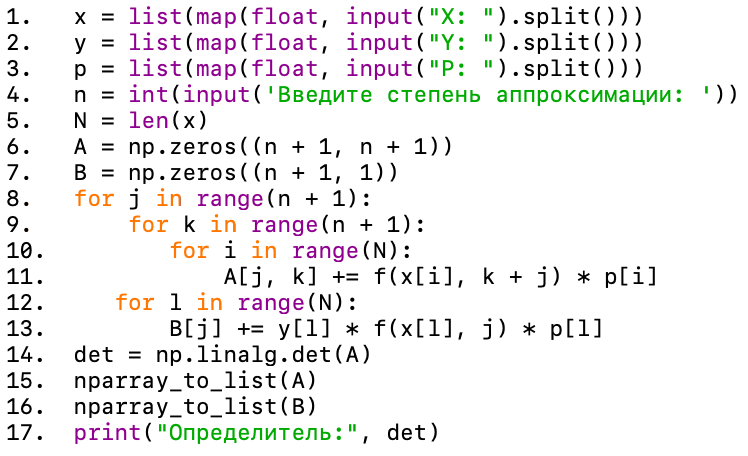
\includegraphics[scale=1.3]{img/code.png}}
		\caption{Пронумерованные строки кода}
		\label{ris:image_code}
	\end{figure}

	\chapter{Графовые модели}
	
	\section{Граф управления}
	
		\begin{figure}[H]	
					\centering	
		{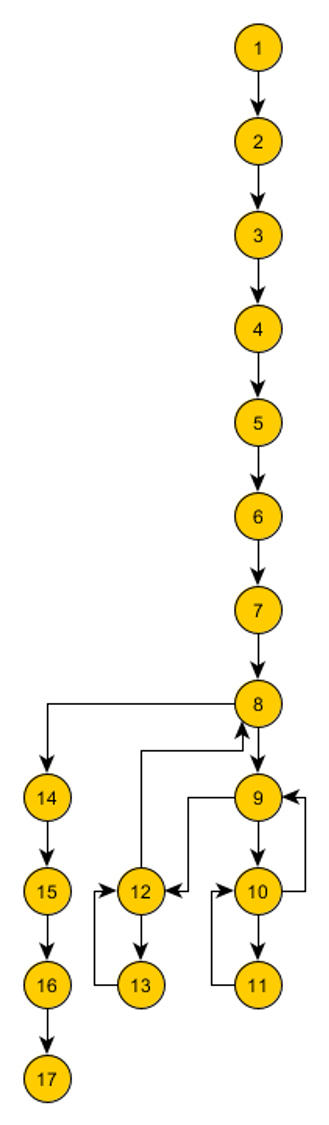
\includegraphics[scale=0.8]{img/gu.png}}
		\caption{Пронумерованные строки кода}
	\end{figure}

	\section{Операционная история}
	
		\begin{figure}[H]	
					\centering	
		{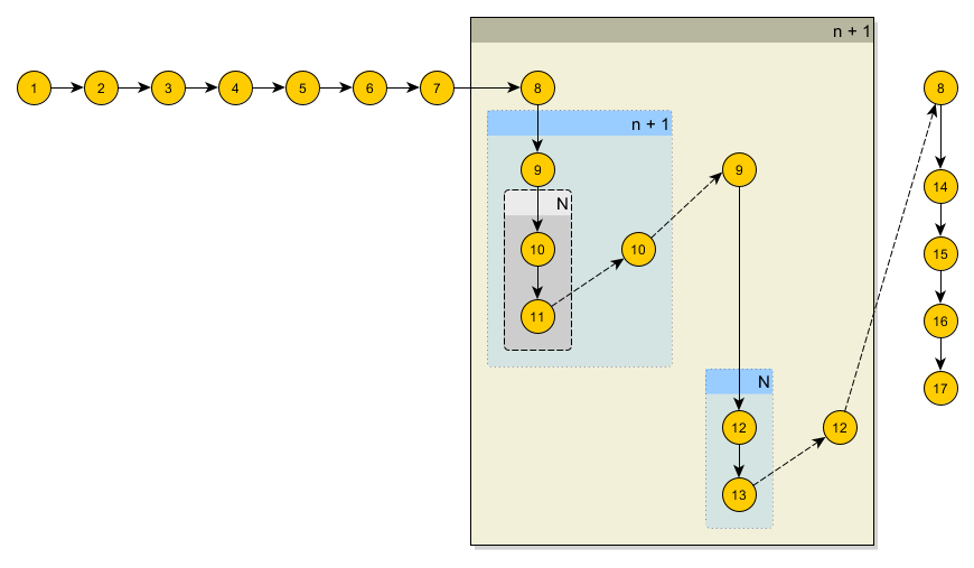
\includegraphics[scale=1.1]{img/oi.png}}
		\caption{Пронумерованные строки кода}
	\end{figure}

	\section{Информационный граф}
		\begin{figure}[H]	
					\centering	
		{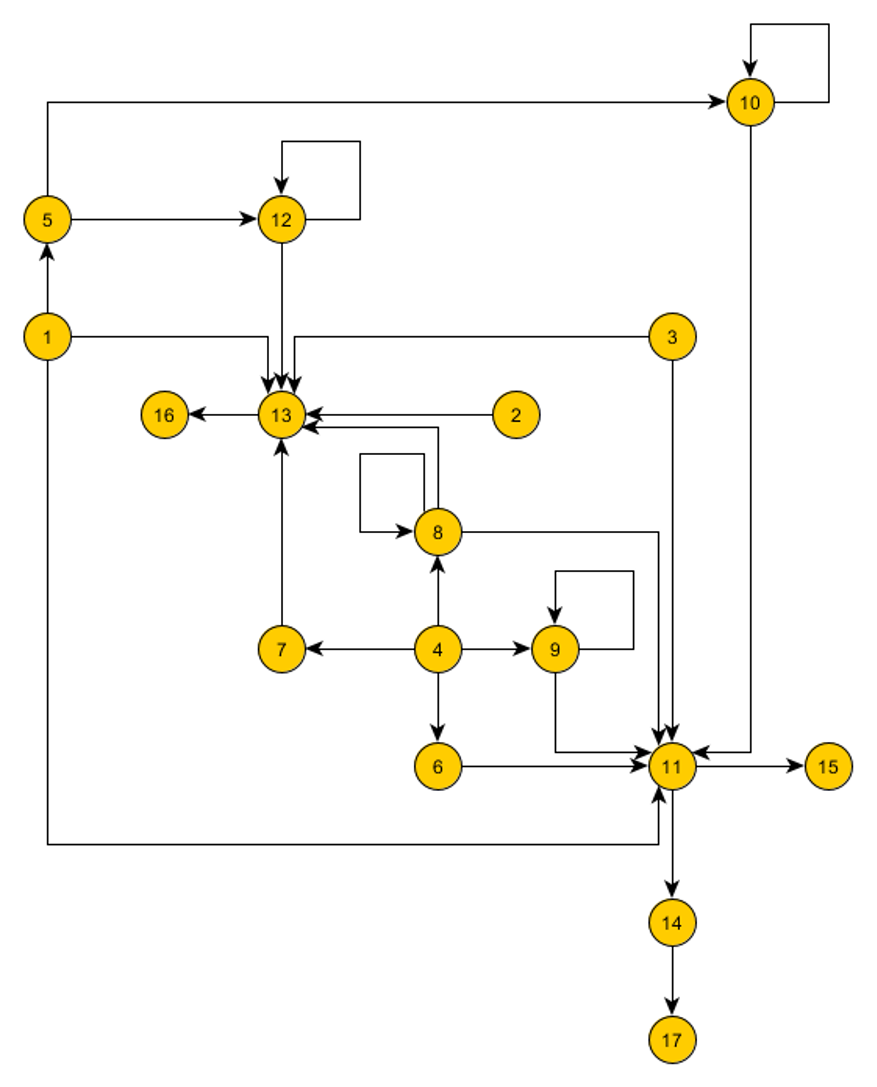
\includegraphics[scale = 1]{img/ig.png}}
		\caption{Пронумерованные строки кода}
	\end{figure}

	\section{Информационная история}
	Для очередных итераций внешнего цикла (вершина 8) в модели не были указаны дуги связей с целью сохранения наглядности графа (в частности, не указаны дуги связи для вершин 9, 10, 11, 12, 13, получаемые аналогично первой итерации из вершин 1, 2, 3, 4, 5, 6, 7).
	\begin{figure}[H]	
				\centering	
	{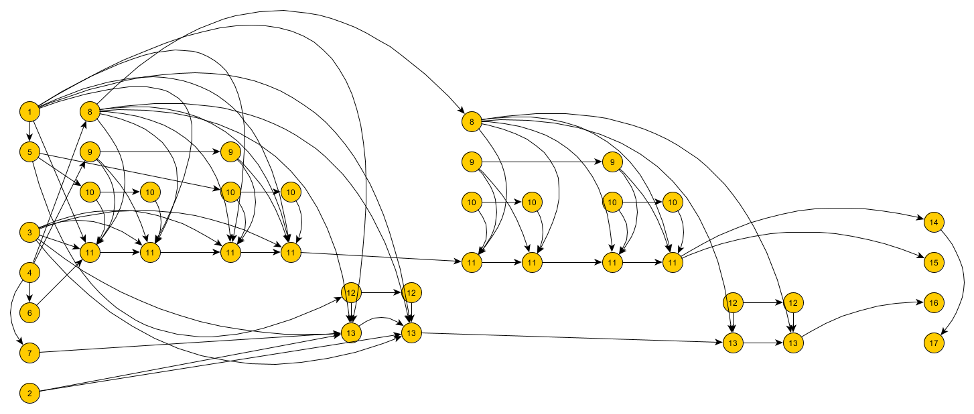
\includegraphics[scale = 1.15]{img/ii.png}}
	\caption{Пронумерованные строки кода}
	\end{figure}
	
	
\end{document}